\documentclass[tikz,border=10pt]{standalone}
\begin{document}
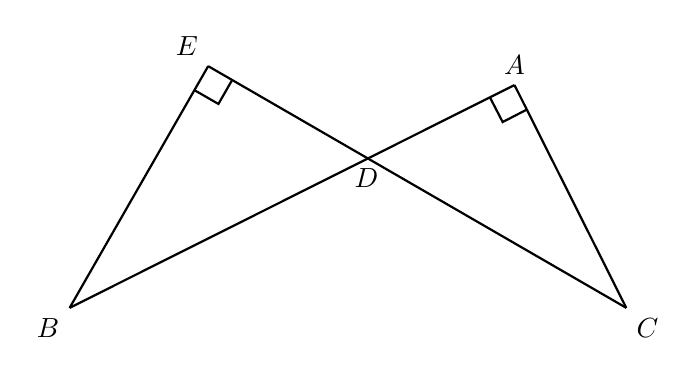
\begin{tikzpicture}[line width=0.8pt]
  \coordinate (B) at (0,0);
  \coordinate (C) at (7.07,0);
  \coordinate (A) at (5.65,2.83);
  \coordinate (E) at (1.76,3.07);
  \coordinate (D) at (3.77,1.90);

  \draw (B) -- (E);
  \draw (E) -- (C);
  \draw (B) -- (A);
  \draw (A) -- (C);

  % right angle mark at E
  \draw (1.585,2.765) -- (1.89,2.59) -- (2.065,2.895);
  % right angle mark at A
  \draw (5.34,2.67) -- (5.50,2.36) -- (5.81,2.52);

  \node[below left] at (B) {$B$};
  \node[below right] at (C) {$C$};
  \node[above] at (A) {$A$};
  \node[above left] at (E) {$E$};
  \node[below] at (D) {$D$};
\end{tikzpicture}
\end{document}
